\documentclass[11pt,a4paper]{article}

\usepackage[utf8]{inputenc}
\usepackage[T1]{fontenc}
\usepackage[a4paper,margin=2.5cm]{geometry}
\usepackage{xcolor}
\usepackage{graphicx}
\usepackage{booktabs}
\usepackage{array}
\usepackage{hyperref}
\usepackage{listings}

\definecolor{codebg}{RGB}{245,247,250}
\definecolor{codeframe}{RGB}{190,198,210}
\definecolor{linkblue}{RGB}{25,75,130}
\hypersetup{colorlinks=true,linkcolor=linkblue,urlcolor=linkblue,
  pdftitle={Laboratorio OpenSSH},pdfauthor={Jorgr Arévalo y Jon González}}
\lstset{basicstyle=\ttfamily\small,backgroundcolor=\color{codebg},frame=single,
  rulecolor=\color{codeframe},columns=fullflexible,keepspaces=true,
  breaklines=true,showstringspaces=false}

\title{Laboratorio OpenSSH}
\author{Jorgr Arévalo \and Jon González}
\date{2 de octubre de 2026}

\begin{document}
\begin{titlepage}
  \centering
  \vspace*{2cm}
  {\Large Sistemas de Redes y Servicios de Internet\par}
  \vspace{1.5cm}
  {\Huge\bfseries Laboratorio OpenSSH\par}
  \vspace{1cm}
  {\large Análisis de conexiones, reenvío de puertos y autenticación\par}
  \vfill
  {\large Jorgr Arévalo\\Jon González\par}
  \vspace{0.8cm}
  {\large 2 de octubre de 2026\par}
\end{titlepage}
\tableofcontents
\newpage

\section{Introducción}
El objetivo de este laboratorio es estudiar el funcionamiento de OpenSSH y
compararlo con una conexión Telnet. En esta entrega se documentan únicamente
las pruebas realizadas hasta el momento: preparación de Telnet, observación de
los puertos, análisis de una conexión SSH en modo verbose, reenvío local de
puertos y autenticación mediante clave pública.

Los ejercicios de gestión de claves con \texttt{ssh-agent} y de una
funcionalidad adicional de OpenSSH no se incluyen, porque todavía no se dispone
de resultados o capturas de esas pruebas.

\section{Entorno y preparación}
Las pruebas se realizaron en Debian GNU/Linux, en la máquina
\texttt{bocata-jamon}, utilizando los usuarios \texttt{user1} y
\texttt{user2}. La versión observada fue OpenSSH 10.0p2, sobre el núcleo
\texttt{6.12.107+deb13-amd64}.

Se instalaron Telnet y su servidor:
\begin{lstlisting}[language=bash]
user1@bocata-jamon:~$ sudo apt install telnet telnetd
\end{lstlisting}
Después se descomentó en \texttt{/etc/inetd.conf} la siguiente línea:
\begin{lstlisting}
telnet stream tcp nowait root /usr/sbin/tcpd /usr/sbin/telnetd
\end{lstlisting}
Finalmente se reinició el servicio:
\begin{lstlisting}[language=bash]
user1@bocata-jamon:~$ sudo systemctl restart inetd
\end{lstlisting}
La salida de \texttt{ss -tan} confirmó que SSH escuchaba en el puerto 22 y
Telnet en el puerto 23:
\begin{lstlisting}
user1@bocata-jamon:~$ ss -tan
LISTEN 0 128 0.0.0.0:22 0.0.0.0:*
LISTEN 0 10  0.0.0.0:23 0.0.0.0:*
LISTEN 0 128 [::]:22    [::]:*
user1@bocata-jamon:~$
\end{lstlisting}

\section{Comparación entre Telnet y SSH con Wireshark}
Se preparó Wireshark para escuchar en la interfaz de loopback. La conexión
Telnet transmite la sesión sin cifrado, por lo que el contenido de la
conversación puede observarse al seguir el flujo TCP. SSH, en cambio, negocia
los algoritmos criptográficos y, después del intercambio de claves y de
\texttt{SSH2\_MSG\_NEWKEYS}, protege el contenido de la sesión.

En las pruebas se utilizó la opción de Wireshark \emph{Follow Stream} sobre el
flujo correspondiente a SSHv2. Las capturas de Wireshark se añadirán a esta
sección cuando estén disponibles; no se simulan aquí resultados que no han
sido aportados.

\section{Ejercicio 1: conexión SSH en modo verbose}
\subsection{Procedimiento}
Se realizaron las siguientes conexiones desde \texttt{user1} hacia
\texttt{user2}:
\begin{lstlisting}[language=bash]
user1@bocata-jamon:~$ ssh -v user2@localhost
user1@bocata-jamon:~$ ssh -vv user2@localhost
\end{lstlisting}
El cliente resolvió \texttt{localhost} como \texttt{::1} y conectó con el
puerto 22. En ambos casos la conexión terminó correctamente después de
introducir la contraseña de \texttt{user2}.

\subsection{Clasificación de los mensajes}
Los mensajes observados se pueden clasificar según los componentes de SSH:
\begin{center}
\begin{tabular}{>{\raggedright\arraybackslash}p{0.29\linewidth} p{0.60\linewidth}}
\toprule
\textbf{Componente} & \textbf{Mensajes y significado}\\
\midrule
Transporte SSH & El cliente y el servidor anuncian SSH-2.0. Se seleccionan
\texttt{mlkem768x25519-sha256}, la clave de host \texttt{ssh-ed25519} y el
cifrado \texttt{chacha20-poly1305@openssh.com}.\\
\addlinespace
Intercambio de claves & \texttt{SSH2\_MSG\_KEXINIT} y
\texttt{SSH2\_MSG\_KEX\_ECDH\_REPLY} muestran la negociación de algoritmos y
el intercambio de material criptográfico.\\
\addlinespace
Clave del servidor & El cliente comprueba que la clave ED25519 coincide con la
registrada para \texttt{localhost} en \texttt{~/.ssh/known\_hosts}.\\
\addlinespace
Autenticación & El servidor anuncia los métodos \texttt{publickey,password}.
Como no había una clave utilizable, el cliente continúa con contraseña.\\
\addlinespace
Sesión SSH & Tras \texttt{SSH2\_MSG\_NEWKEYS} se abre el canal de sesión, se
solicita una pseudo-terminal y se inicia la shell remota.\\
\bottomrule
\end{tabular}
\end{center}
El modo \texttt{-vv} añade información más detallada sobre las propuestas de
algoritmos, el canal 0, la solicitud de pseudo-terminal y la confirmación de la
shell. Al cerrar la sesión se observan el cierre del canal y el código de salida
0.

\subsection{Resultado}
La conexión se estableció correctamente. El análisis muestra que SSH separa la
negociación criptográfica, la autenticación y la apertura de la sesión. La
contraseña se introduce después de establecer el canal protegido, por lo que
no queda expuesta como texto legible en la red.

\section{Ejercicio 2: comprobación de la clave del host}

En esta prueba se compararon dos estados del cliente SSH:
\texttt{ssh1}, que corresponde a la versión configurada, y \texttt{ssh2}, que
corresponde a la versión instalada de cero.

Las principales diferencias, en orden de aparición al utilizar la opción
\texttt{-v}, fueron las siguientes:
\begin{itemize}
  \item Al inicio, \texttt{ssh1} lee la configuración en
  \texttt{/etc/ssh/ssh\_config}, en
  \path{/etc/ssh/ssh_config.d/20-systemd-ssh-proxy.conf} y aplica la
  configuración.
  \item \texttt{ssh2} muestra un par de veces un error de \texttt{fopen} al
  intentar abrir \texttt{.ssh/known\_hosts}.
  \item \texttt{ssh1} comprueba que ``localhost'' es un host conocido y que se
  corresponde con la clave ED25519.
  \item \texttt{ssh2}, en ese mismo punto, busca los ficheros que contienen
  firmas de hosts y, al no encontrarlos, determina que no se puede comprobar la
  autenticidad del host.
  \item \texttt{ssh2} avisa al usuario de que no se conoce la clave y pregunta
  si quiere continuar.
  \item \texttt{ssh2} avisa de que el soporte de SELinux está deshabilitado.
  \item \texttt{ssh2} muestra un aviso de que el host ``localhost'' se ha
  añadido permanentemente a la lista de \texttt{known\_hosts}.
  \item \texttt{ssh1} avisa de que no hay ninguna clave del servidor nueva o
  revocada y carga las variables de entorno \texttt{COLORTERM} y
  \texttt{LANG}.
  \item \texttt{ssh2}, en ese punto, avisa de que ha aprendido nuevas claves
  del host y que las ha guardado.
\end{itemize}

Al intentar conectarse, como ya no se tenían guardadas las claves del host, SSH
avisó de que no se podía determinar la autenticidad del host, mostró la clave
ED25519 y preguntó si se quería continuar. Al responder afirmativamente, guardó
la clave.

\section{Ejercicio 3: reenvío local de puertos}
\subsection{Configuración del túnel}
Desde la máquina local se ejecutó:
\begin{lstlisting}[language=bash]
user1@bocata-jamon:~$ ssh -L 12000:ehu.eus:443 user1@SRDSI
\end{lstlisting}
La opción \texttt{-L} crea un puerto local, el 12000, cuyo tráfico se envía a
través de SSH hacia \texttt{ehu.eus:443}. El túnel se comprobó mediante:
\begin{lstlisting}[language=bash]
user1@bocata-jamon:~$ sudo netstat -tanp | grep 12000
tcp 0 0 127.0.0.1:12000 0.0.0.0:* LISTEN 324823/ssh
tcp6 0 0 ::1:12000       :::*              LISTEN 324823/ssh
\end{lstlisting}
La salida muestra que un proceso \texttt{ssh} estaba escuchando en
\texttt{127.0.0.1:12000} y en \texttt{::1:12000}.

\subsection{Prueba desde Firefox}
Se intentó acceder a \texttt{localhost:12000} desde Firefox antes y después de
establecer el túnel.

\begin{figure}[htbp]
  \centering
  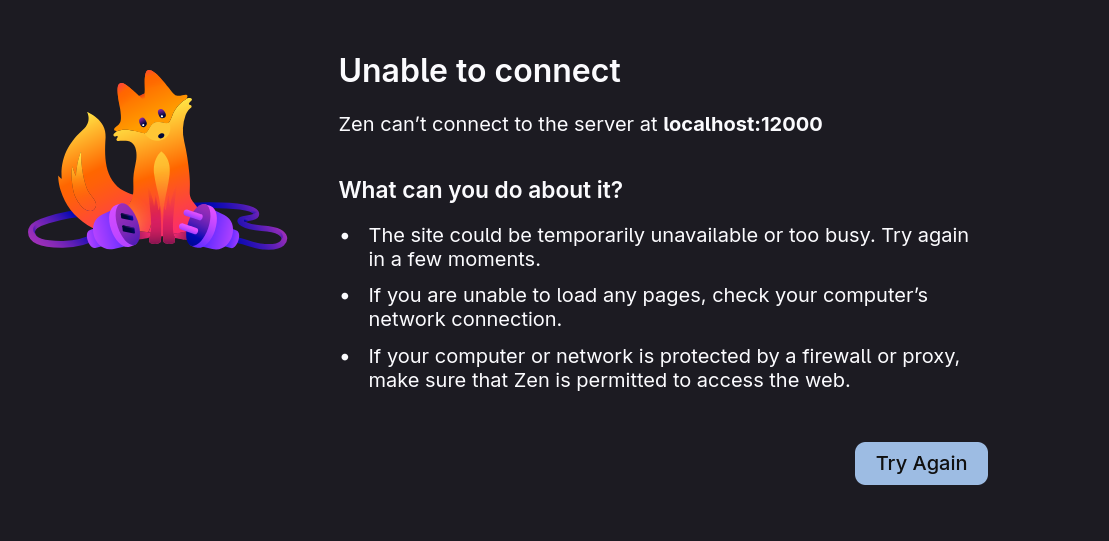
\includegraphics[width=0.88\linewidth]{firefox-notunnel.png}
  \caption{Intento de conexión a \texttt{localhost:12000} sin el túnel.}
  \label{fig:notunnel}
\end{figure}

Sin el túnel, Firefox mostró ``Unable to connect'' y no pudo conectarse al
servidor en \texttt{localhost:12000} (figura~\ref{fig:notunnel}).

\begin{figure}[htbp]
  \centering
  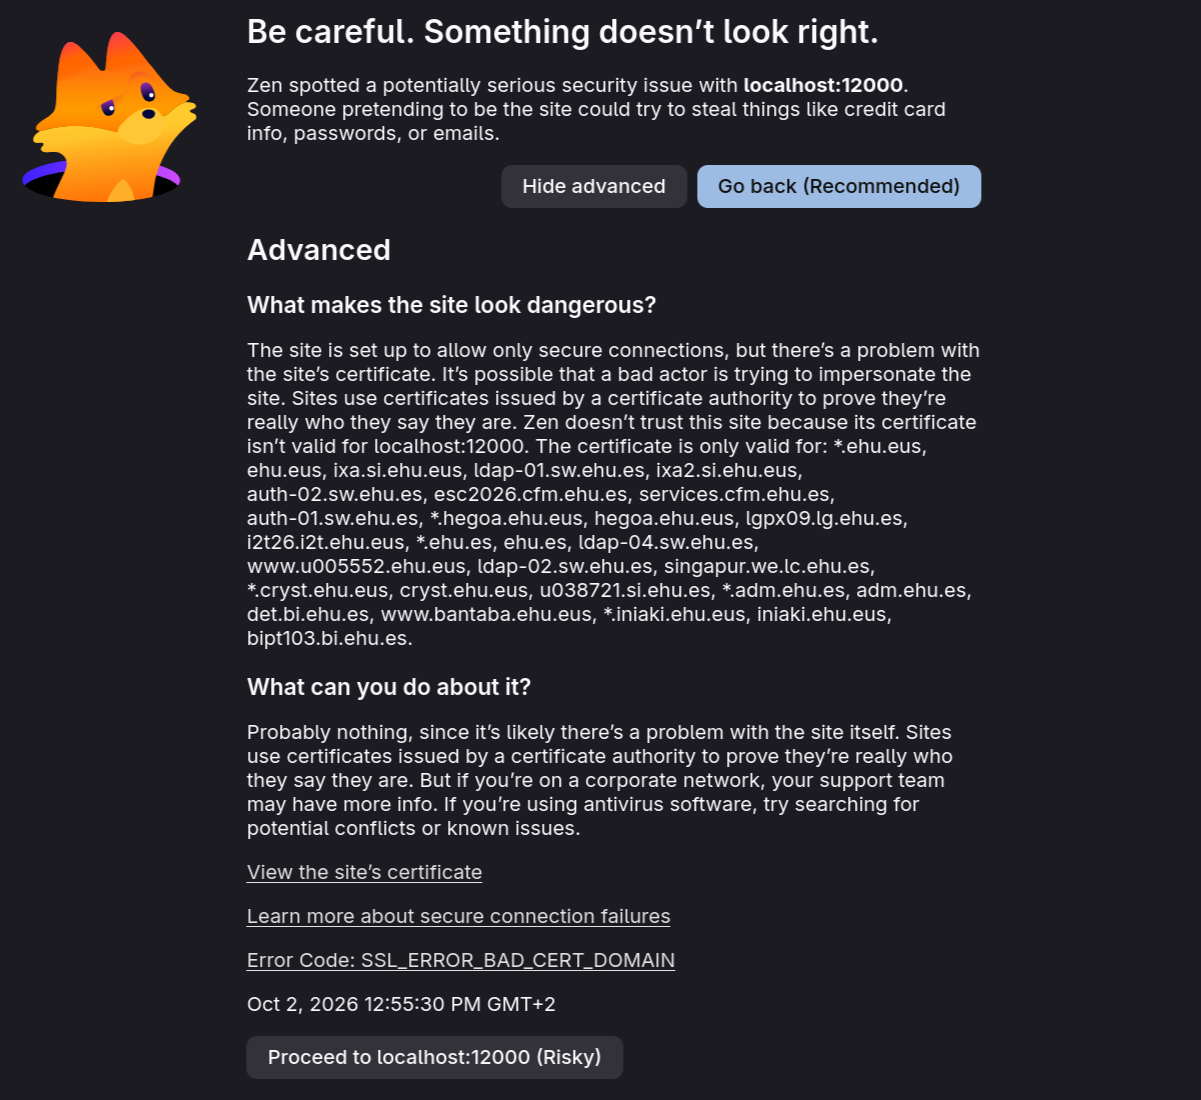
\includegraphics[width=0.88\linewidth]{firefox-withtunnel.png}
  \caption{Intento de conexión a \texttt{localhost:12000} con el túnel.}
  \label{fig:withtunnel}
\end{figure}

Con el túnel activo, Firefox recibió una respuesta HTTPS, pero mostró el error
\texttt{SSL\_ERROR\_BAD\_CERT\_DOMAIN}. La pantalla indica que el certificado
es válido para nombres de \texttt{ehu.eus}, no para \texttt{localhost:12000}.
Por tanto, la captura demuestra que se alcanzó el servicio HTTPS remoto a través
 del reenvío, pero la navegación no terminó con una página cargada debido a la
comprobación del nombre del certificado.

\section{Ejercicio 4: autenticación mediante clave pública}
Primero se comprobó que la conexión de \texttt{user1} a \texttt{user2} pedía la
contraseña:
\begin{lstlisting}[language=bash]
user1@bocata-jamon:~$ ssh user2@localhost
\end{lstlisting}
Después se generó para \texttt{user1} un par de claves ED25519:
\begin{lstlisting}[language=bash]
user1@bocata-jamon:~$ ssh-keygen
\end{lstlisting}
La clave privada se guardó en \texttt{~/.ssh/id\_ed25519} y la pública en
\texttt{~/.ssh/id\_ed25519.pub}. La clave pública se copió a la cuenta remota
con:
\begin{lstlisting}[language=bash]
user1@bocata-jamon:~$ ssh-copy-id user2@localhost
\end{lstlisting}
Este comando pidió la contraseña para instalar la clave en
\texttt{~user2/.ssh/authorized\_keys}. Después, al ejecutar de nuevo
\texttt{ssh user2@localhost}, la conexión se realizó sin pedir la contraseña de
la cuenta remota. Solo se copió la clave pública; la clave privada permaneció en
\texttt{user1}.

\section{Conclusiones}
Las pruebas realizadas muestran la diferencia principal entre Telnet y SSH:
Telnet no cifra la sesión, mientras que SSH negocia algoritmos criptográficos,
verifica la identidad del servidor y protege la autenticación y la sesión.

También se comprobó el reenvío local de puertos. Sin el túnel, el puerto local
12000 no aceptaba la conexión. Con el túnel, la petición llegó al servicio
HTTPS de \texttt{ehu.eus}; el error observado se debió a que el certificado
remoto no corresponde al nombre \texttt{localhost}. Finalmente, la
autenticación mediante clave pública permitió conectarse sin introducir de
nuevo la contraseña de \texttt{user2}.

\end{document}
